%% start of file `template.tex'.
%% Copyright 2006-2015 Xavier Danaux (xdanaux@gmail.com).
%
% This work may be distributed and/or modified under the
% conditions of the LaTeX Project Public License version 1.3c,
% available at http://www.latex-project.org/lppl/.

\documentclass[11pt,a4paper,sans]{moderncv}        % possible options include font size ('10pt', '11pt' and '12pt'), paper size ('a4paper', 'letterpaper', 'a5paper', 'legalpaper', 'executivepaper' and 'landscape') and font family ('sans' and 'roman')

% moderncv themes
\moderncvstyle{banking}                             % style options are 'casual' (default), 'classic', 'banking', 'oldstyle' and 'fancy'
\moderncvcolor{black}                               % color options 'black', 'blue' (default), 'burgundy', 'green', 'grey', 'orange', 'purple' and 'red'
%\renewcommand{\familydefault}{\sfdefault}         % to set the default font; use '\sfdefault' for the default sans serif font, '\rmdefault' for the default roman one, or any tex font name
%\nopagenumbers{}                                  % uncomment to suppress automatic page numbering for CVs longer than one page

% character encoding
\usepackage[utf8]{inputenc}                       % if you are not using xelatex ou lualatex, replace by the encoding you are using

% adjust the page margins
\usepackage[scale=0.75]{geometry}
%\setlength{\hintscolumnwidth}{3cm}                % if you want to change the width of the column with the dates
%\setlength{\makecvtitlenamewidth}{10cm}           % for the 'classic' style, if you want to force the width allocated to your name and avoid line breaks. be careful though, the length is normally calculated to avoid any overlap with your personal info; use this at your own typographical risks...

\usepackage{pdfpages}

% personal data
\name{Luke}{Kokoftopoulos}
% \title{Resumé title}                               % optional, remove / comment the line if not wanted
\address{Software Engineer}{University of Technology Sydney}% optional, remove / comment the line if not wanted; the "postcode city" and "country" arguments can be omitted or provided empty
\phone[mobile]{0478 790 532}                   % optional, remove / comment the line if not wanted; the optional "type" of the phone can be "mobile" (default), "fixed" or "fax"
% \phone[fixed]{+2~(345)~678~901}
% \phone[fax]{+3~(456)~789~012}
\email{luke.d.kokoftopoulos@student.uts.edu.au}                               % optional, remove / comment the line if not wanted
% \homepage{www.johndoe.com}                         % optional, remove / comment the line if not wanted
\social[linkedin]{lukekoko}                        % optional, remove / comment the line if not wanted
% \social[twitter]{jdoe}                             % optional, remove / comment the line if not wanted
\social[github]{lukekoko}                              % optional, remove / comment the line if not wanted
% \extrainfo{additional information}                 % optional, remove / comment the line if not wanted
% \photo[64pt][0.4pt]{picture}                       % optional, remove / comment the line if not wanted; '64pt' is the height the picture must be resized to, 0.4pt is the thickness of the frame around it (put it to 0pt for no frame) and 'picture' is the name of the picture file
% \quote{Some quote}                                 % optional, remove / comment the line if not wanted

% bibliography adjustements (only useful if you make citations in your resume, or print a list of publications using BibTeX)
%   to show numerical labels in the bibliography (default is to show no labels)
\makeatletter\renewcommand*{\bibliographyitemlabel}{\@biblabel{\arabic{enumiv}}}\makeatother
%   to redefine the bibliography heading string ("Publications")
%\renewcommand{\refname}{Articles}

% bibliography with mutiple entries
%\usepackage{multibib}
%\newcites{book,misc}{{Books},{Others}}
%----------------------------------------------------------------------------------
%            content
%----------------------------------------------------------------------------------
\begin{document}
%-----       resume       ---------------------------------------------------------
\makecvtitle

\section{Education}
\cventry{January 2017--November 2021}{Bachelor of Engineering(Honours) in Software}{University of Technology Sydney}{}{}{Sub-major in Data Analytics with a focus in Machine Learning}  % arguments 3 to 6 can be left empty
\cventry{January 2017--November 2021}{Diploma in Professional Engineering Practice}{University of Technology Sydney}{}{}{}  % arguments 3 to 6 can be left empty

\section{Engineering Capstone}
\cvitem{Title}{\emph{Software Security Analysis using Deep Learning}}
\cvitem{Supervisors}{Yulei Sui}
\cvitem{Description}{The project aim is to develop new techniques to detect and repair software security vulnerabilities for large and real-world software projects by leveraging deep learning and natural language processing.}

\section{Experience}
% \subsection{Vocational}
\cventry{February 2020--Current}{Junior Support Engineer}{GTSGroup}{}{}{
\begin{itemize}%
\item OSIsoft PI Systems support for various clients.
\item Developing various ETL(Extract, transform, load) Python scripts for clients.
\item Working in a project team to setup, install and customise the PI System for clients.
\end{itemize}}
\cventry{January 2019--January 2020}{Engineer Undergraduate - Software}{Veolia Australia and New Zealand}{}{}{
\begin{itemize}%
\item Developed various Python scripts for ETL, web scraping, automation and data processing.
\item Developed web application using Angular and Node.js for internal use. 
\item Maintaining OSIsoft PI System.
\end{itemize}}


\cventry{August 2018-- January 2019}{Software Engineering Intern}{Veolia Australia and New Zealand}{}{}{
\begin{itemize}%
\item Developed various Python scripts for ETL, web scraping, automation and data processing.
\item Developed web application using Angular and Node.js for internal use. 
\item Maintaining OSIsoft PI System.
\end{itemize}}

\section{Technical Skills}
\cvitemwithcomment{Programming}{Python, JavaScript, TypeScript, C, C++, C\#, Java, SQL}{}
\cvitemwithcomment{Web Development}{Angular, React, Node.js, Docker, GCP, Firebase, AWS}{}
\cvitemwithcomment{Data Science}{TensorFlow, Keras, Pandas, Scikit-Learn, NumPy}{}
\cvitemwithcomment{Tools}{Git, GitHub, Travis CI, Excel, Jira, Trello}{}
\cvitemwithcomment{Systems}{OSIsoft PI System; PI AF, PI Vison, PI Web API, PI UFL interface, PI Datalink}{}

\section{Transferable Skills}
\cvlistitem{Strong \textbf{problem solving} skill demonstrated by being a system support engineer. I regularly solve various customer problems relating to systems issues. I have also developed many ETL scripts that solve problems with data ingest.}
\cvlistitem{Ability to work in a \textbf{team} and \textbf{independently} shown through employment at GTSGroup and Veolia. I have also worked in a variety of teams in 6 Software Engineering Studios at university where I got a high distinction mark. }
\cvlistitem{Strong \textbf{communication} and \textbf{listening} skills demonstrated through employment at GTSGroup and Veolia. I communicate through email, phone, online meetings and in person to colleagues and clients.}
\cvlistitem{\textbf{Fast learner} shown by the ability to learn new tools and software quickly. I am constantly learning new software libraries and frameworks at work and university.}
\cvlistitem{Efficient \textbf{time management} shown by completing system support tickets within the resolution time at GTSGroup.}

% \section{References}
% \begin{cvcolumns}
%   \cvcolumn{Category 1}{\begin{itemize}\item Person 1\item Person 2\item Person 3\end{itemize}}
%   \cvcolumn{Category 2}{Amongst others:\begin{itemize}\item Person 1, and\item Person 2\end{itemize}(more upon request)}
%   \cvcolumn[0.5]{All the rest \& some more}{\textit{That} person, and \textbf{those} also (all available upon request).}
% \end{cvcolumns}

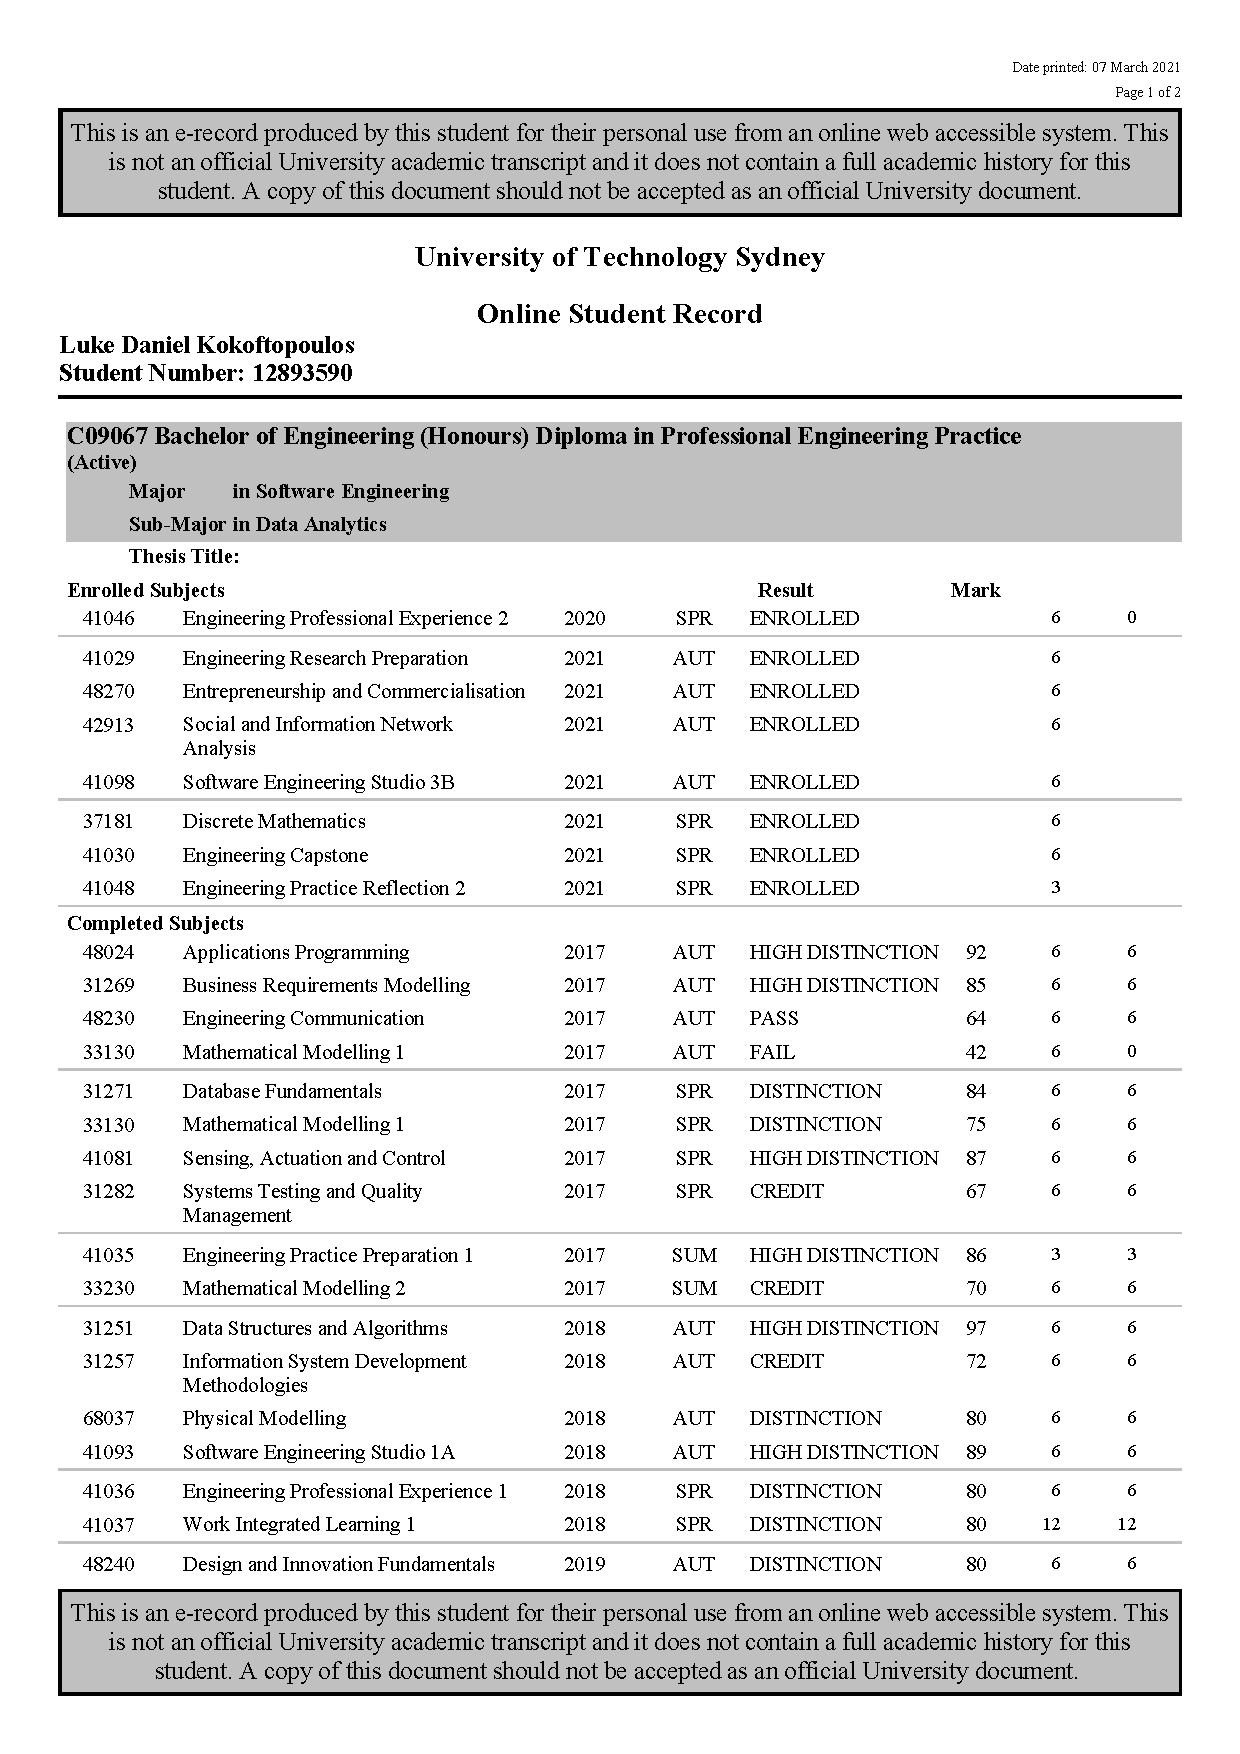
\includepdf[pages=-]{transcript.pdf}

\clearpage
\end{document}


%% end of file `template.tex'.
